\documentclass[11pt]{beamer}
\usetheme{Boadilla}
\usepackage[utf8]{inputenc}
\usepackage{amsmath}
\usepackage{amsfonts}
\usepackage{amssymb}

\title{Taller Ecología del Movimiento}
%\setbeamercovered{transparent} 
%\setbeamertemplate{navigation symbols}{} 
%\logo{} 
%\institute{} 
\date{\today} 
%\subject{} 
\begin{document}

\begin{frame}
\titlepage
\end{frame}

%\begin{frame}
%\tableofcontents
%\end{frame}

\begin{frame}{¿En qué lugar pasas tu día en Ciencias?}
	\begin{figure}
		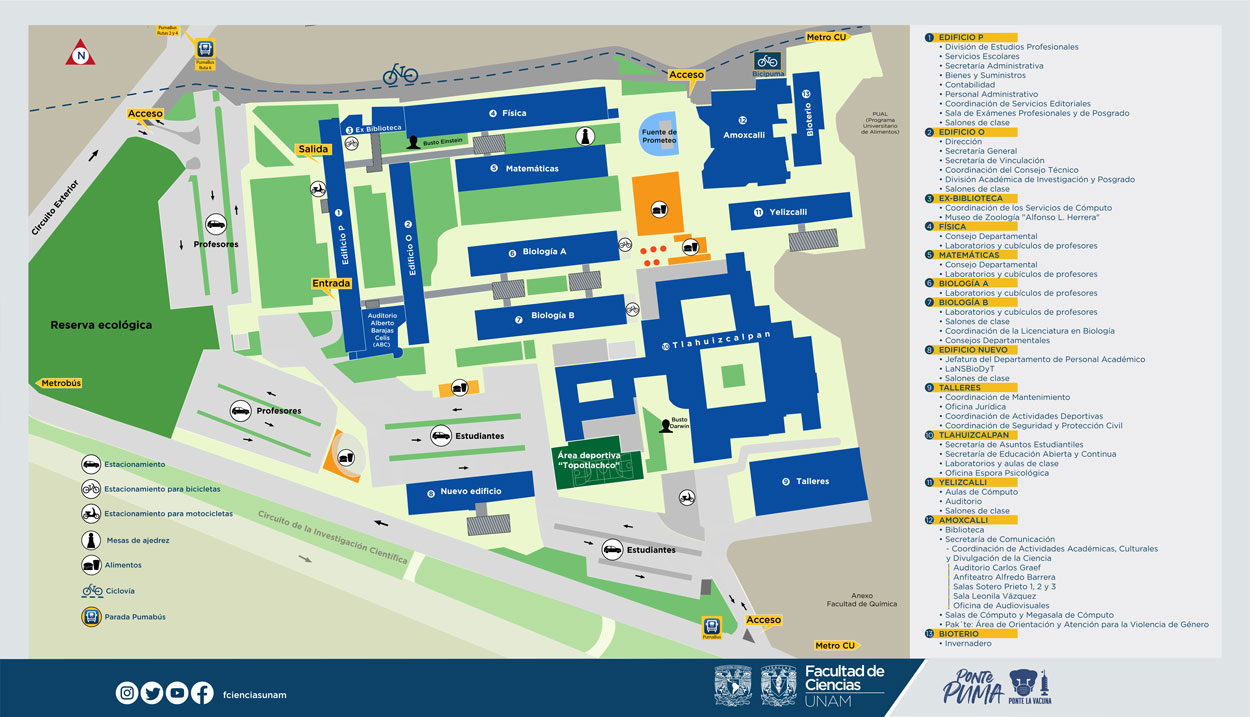
\includegraphics[scale=0.28]{images/MAPA_Fac_2021.jpg}
	\end{figure}
\end{frame}


\begin{frame}{Marco conceptual de la Ecología del Movimiento \cite{nathan2008movement}}

El marco incorpora dos grandes componentes: 
	\begin{itemize}
		\item Componente basado en el individuo.
		\item Componente basado en los factores externos que influyen en las causas, mecanismos y patrones de movimiento.
	\end{itemize}


\end{frame}

\begin{frame}{Componente basado en el individuo}
Preguntas

	\begin{enumerate}
		\item ¿Por qué se mueven?
		\item ¿Dónde se mueven?
		\item ¿Cómo se mueven?			
	\end{enumerate}	

Proceso de toma de decisión de movimiento del individuo :			
				\begin{center}
					 \textbf{¿Cómo se le asigna una importancia relativa al comportamiento de acuerdo a diferentes objetivos como reproducción, alimentación, descanso, etc?¿Cómo entendemos el movimiento de acuerdo a distintas metas o propositos?}
				\end{center}
\end{frame}

\begin{frame}{Componente basado en los factores externos}
	\begin{itemize}
		\item ¿Cómo está cambiando el entorno-contexto donde se desarrolla el individuo?
	\end{itemize}
\end{frame}

\begin{frame}{Tipología de movimiento}

Los principales tipos de movimiento son los de:
	
	\begin{enumerate}
		\item \textbf{Residencia o área de actividad estable} son los movimientos registrados en áreas bien definidas y estables para distintos años. 
		\item \textbf{Migración} es el movimiento estacional-periódico estable de largas distancias entre distintas localidades. Corresponden a movimientos de acuerdo a estaciones del año.
		\item \textbf{Dispersión} es el movimiento en el que la población o individuo deja la localidad ocupada y se mueve hacia una localidad diferente. Ambas áreas, la dejada y la de llegada, son ocupadas por periodos largos de tiempo.
		\item \textbf{Nomadismo} movimiento que tiene una frecuencia alta, no estacional o periódica, y tampoco estable tanto en tiempo de permanencia y de dirección.  
	\end{enumerate}
\end{frame}

\begin{frame}{Net squared displacement (NSD)}
Una forma de distinguir estos tipos de movimientos es mediante el \textbf{Net squared displacement (NSD)}. Este indicador mide la distancia a partir de un punto de inicio de la trayectoria, donde inicia el seguimiento, hasta el punto final de seguimiento.

\end{frame}

\begin{frame}{Migración}
	\begin{figure}
		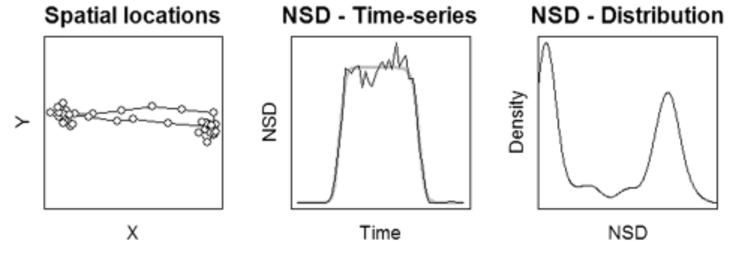
\includegraphics[scale=0.8]{images/migracion}
		\caption{Migración. Tomado de \cite{bastille2016flexible}}
	\end{figure}
\end{frame}


\begin{frame}{Dispersión}
	\begin{figure}
		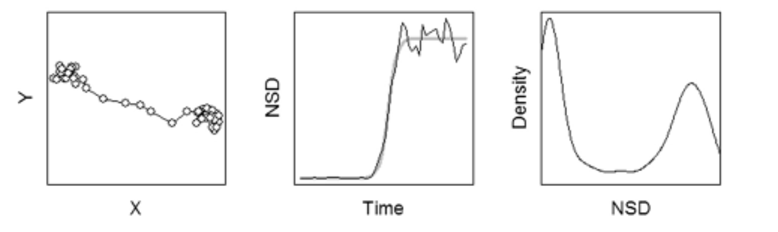
\includegraphics[scale=0.8]{images/dispersion}
		\caption{Dispersión. Tomado de \cite{bastille2016flexible}}
	\end{figure}
\end{frame}


\begin{frame}{Nomadismo}
	\begin{figure}
		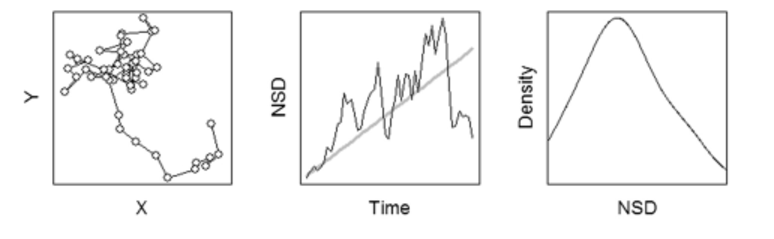
\includegraphics[scale=0.8]{images/nomadismo}
		\caption{Nomadismo. Tomado de \cite{bastille2016flexible}}
	\end{figure}
\end{frame}



\begin{frame}{Sedentarismo}
	\begin{figure}
		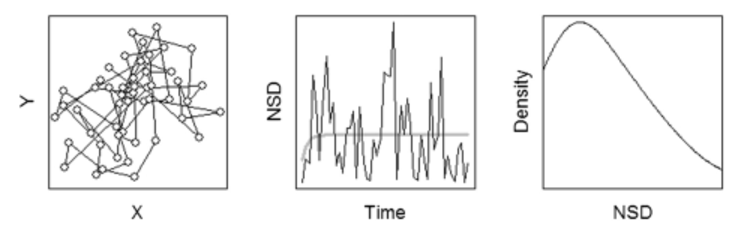
\includegraphics[scale=0.8]{images/sedentarismo}
		\caption{Sedentarismo. Tomado de \cite{bastille2016flexible}}
	\end{figure}
\end{frame}


\begin{frame}{Datos: Movebank for animal tracking data}
	\begin{figure}
		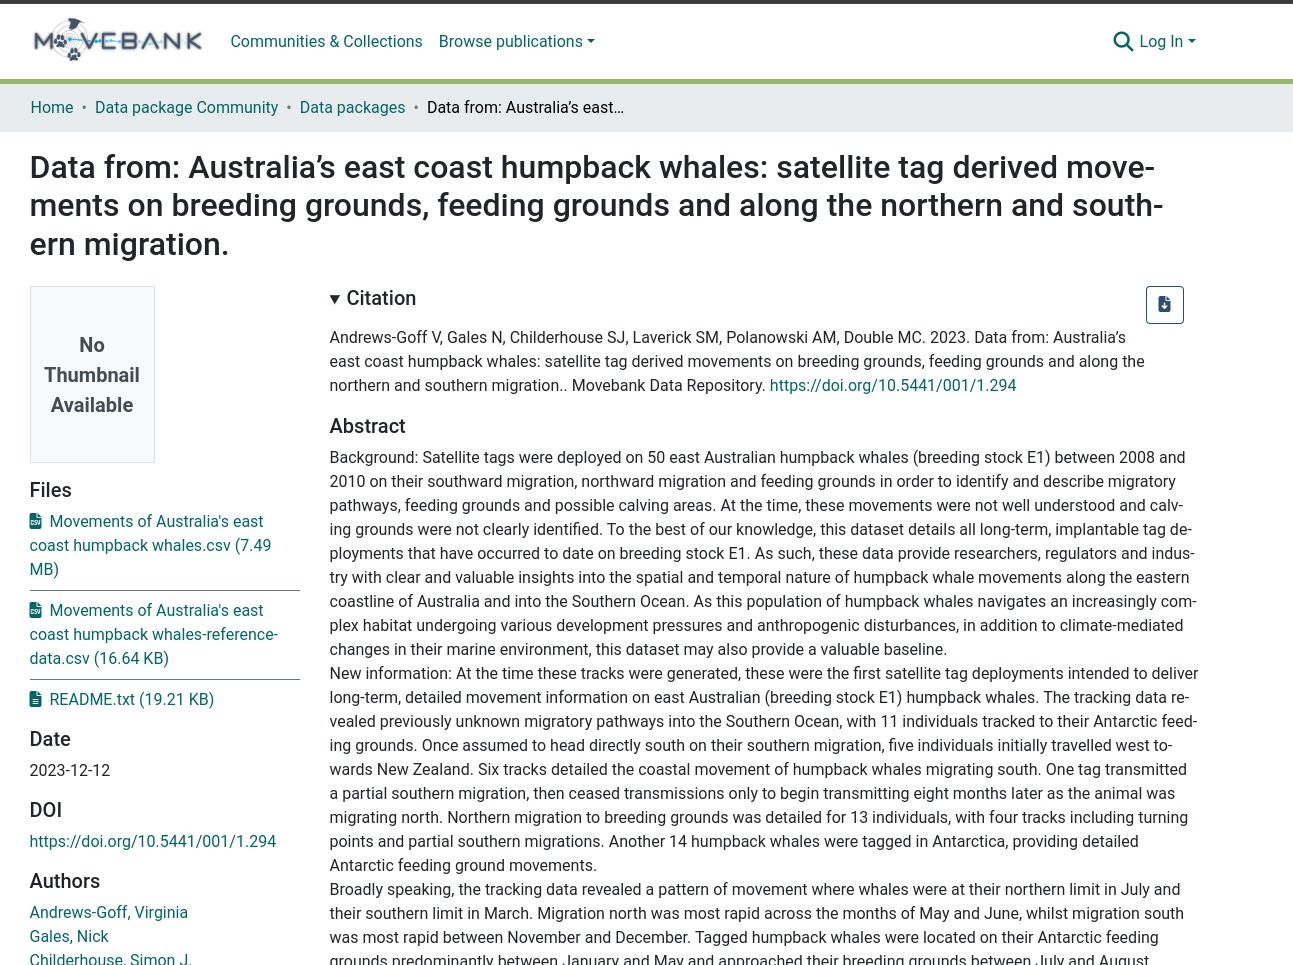
\includegraphics[scale=0.2]{images/losdatos}
		\caption{https://www.movebank.org/}
	\end{figure}
\end{frame}

\begin{frame}{Humpback whales}
	\begin{figure}
		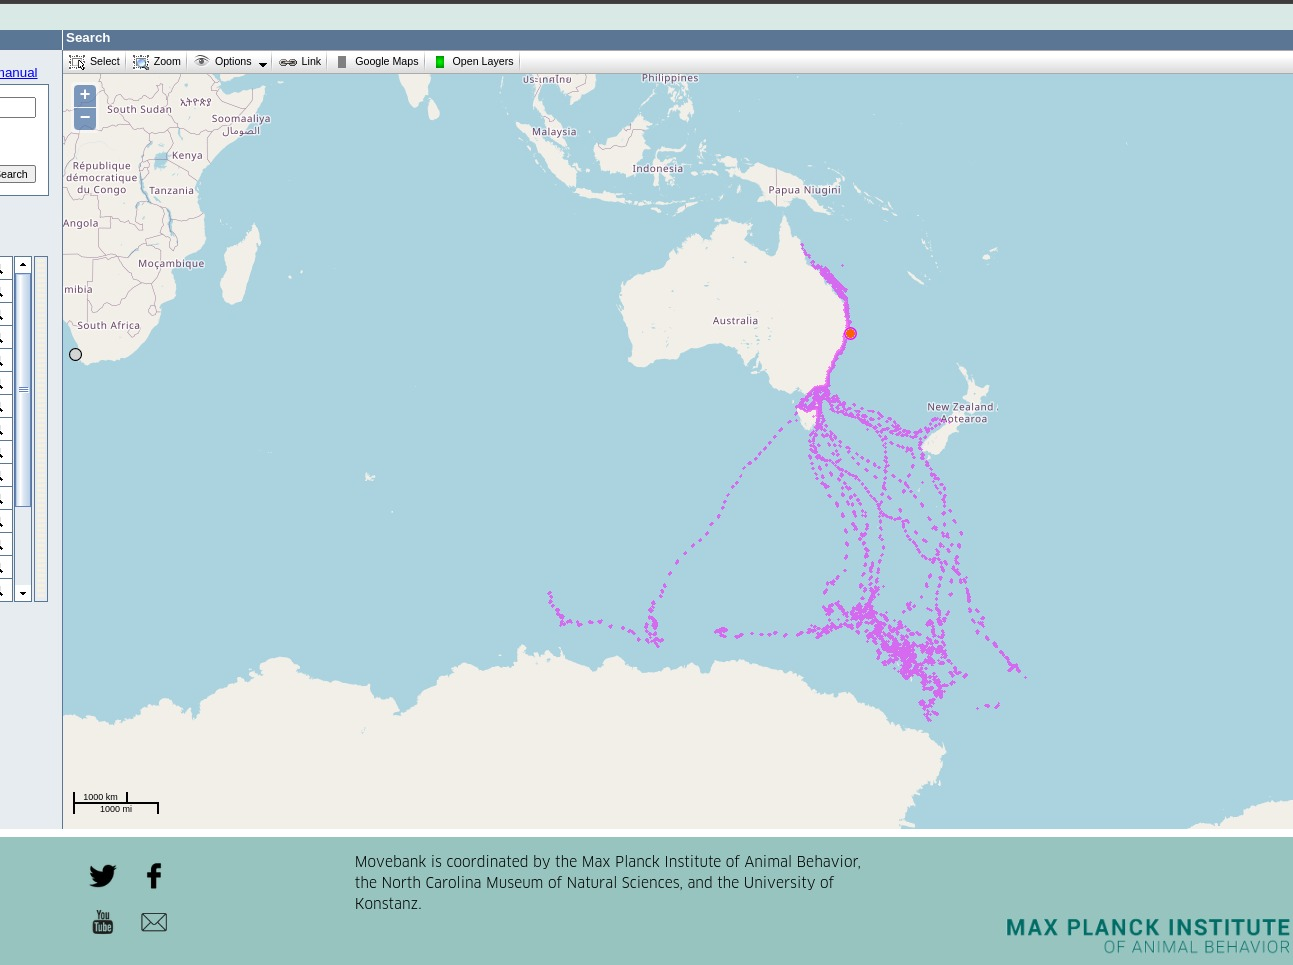
\includegraphics[scale=0.23]{images/elmovimiento}
	\end{figure}
\end{frame}

\begin{frame}{Actividades}
	\begin{itemize}
		\item Calcular Net squared displacement (NSD).
		\item Estimar Kernel Density
	\end{itemize}
\end{frame}

\begin{frame}{Kernel Density Univariado}
	\begin{figure}
		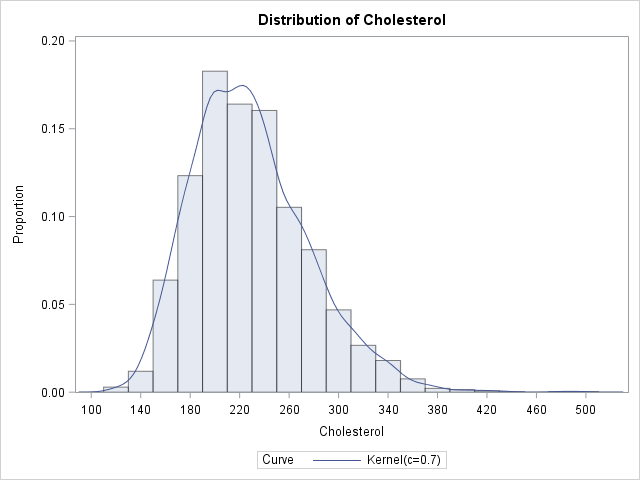
\includegraphics[scale=0.6]{images/KDECholesterol}
	\end{figure}
\end{frame}

\begin{frame}{Kernel Density Bivariado}
	\vspace{-0.2cm}
	\begin{figure}
		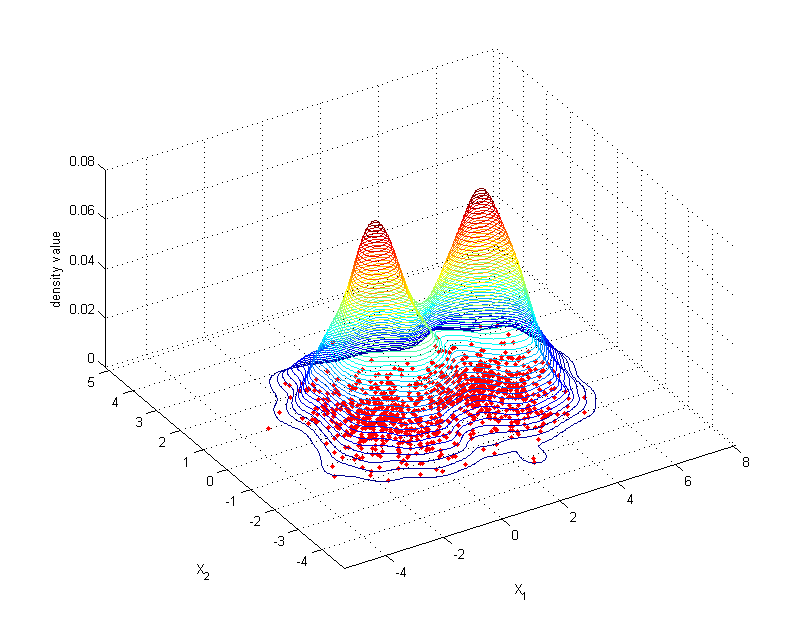
\includegraphics[scale=0.5]{images/Bivariate_example}
	\end{figure}
\end{frame}

\begin{frame}{Referencias}
\bibliographystyle{apalike} 
\bibliography{taller_eco_mov.bib}
\end{frame}

\end{document}